\section{ボール検出}
\label{sec:ball-detection}

\subsection{標準モデルと外部注釈}

標準経路は、i935の時系列検出器でカメラごとに球の位置と存在スコアを推定する。
入力映像から作るMDDは、隣接時刻の変化を符号別に表す差分特徴である。
i935はMDDの\ev{ball-config}{2}チャネルを受け取り、\ev{ball-config}{8}フレームの窓を使う。
同一フレームを複数窓が覆う場合は窓の中心に近い予測を採用し、候補点を運動整合の検査へ渡す。
別設定として、RGBとMDDを入力とするX3D／CSN系の動画エンコーダ\cite{x3d,csn}に
DPT型の高密度デコーダ\cite{dpt}をつないだ\ev{ball-x3d}{32}フレームの球検出器を用意した。
Meiji 4camのclip\_000からcam1〜cam3を使い、X3Dで得たカメラ幾何を両方式に固定して診断した。
有効な球3Dはi935で\ev{ball-x3d}{113/356}、X3Dで\ev{ball-x3d}{123/356}元フレームだった。
校正と向き判定を含む同じ視点の通常実行では、i935はコート向きが決まらず停止した。
固定幾何で球観測を比べた結果と、校正・向き判定を含む処理の成立は別の評価となる。

保存済み注釈を固定の幾何へ渡す経路もある。
Meiji 4camの外部座標初版\ev{ball-origin}{69} JSONは、
Chromeが\ev{ball-origin}{2026年11月24日 01:50:43 UTC}に \texttt{chatgpt.com} から取得した記録のあるZIPと全件バイト一致した。
これは取得経路の来歴であり、初版を生成したモデルと実行IDは保存記録からは確定できなかった。
後続の再注釈は同日\ev{ball-origin}{20:27 JST}にCodex CLIのGPT-6.2 Sol（effort max）で開始し、
clip\_012、clip\_015、clip\_026の出力が公開rev1の対応ファイルと一致した。
初版を以下の球像と可視性の診断に用い、rev1の\ev{ball-origin}{3}本はベンチマークの注釈更新に対応する。

\subsection{球像の大きさ・ブラー・可視性}

Meiji 4camの\ev{ball-footprint}{69}クリップでは元画像が\ev{ball-footprint}{1920×1080}、約\ev{ball-footprint}{59.94} fpsだった。
画面内の観測ラベルからカメラ別・クリップ別に時点を選び、前後画像の中央値で作った背景を引いた。
注釈の周辺にある同符号の残差成分から、短軸分散で円盤相当径を、長短軸の分散差で見かけの伸び（ブラー指標）を求めた。
同じ時点を縮小して測定し、成分の面積やコントラストが足りない場合は欠測とした。
元画像では\ev{ball-footprint}{2,121/2,208}件が測れ、径の中央値は\ev{ball-footprint}{4.00} pxだった。
\ev{ball-footprint}{512×288}では\ev{ball-footprint}{360/2,208}件が測れ、
径の中央値は\ev{ball-footprint}{1.76} pxだった。全サイズで測れた\ev{ball-footprint}{339}件を揃えた比較でも、
縮小に伴って径が小さくなった（図\ref{fig:ball-footprints}）。表\ref{tab:ball-cameras}で視点ごとの差を示す。

\begin{figure}[tbp]
\centering
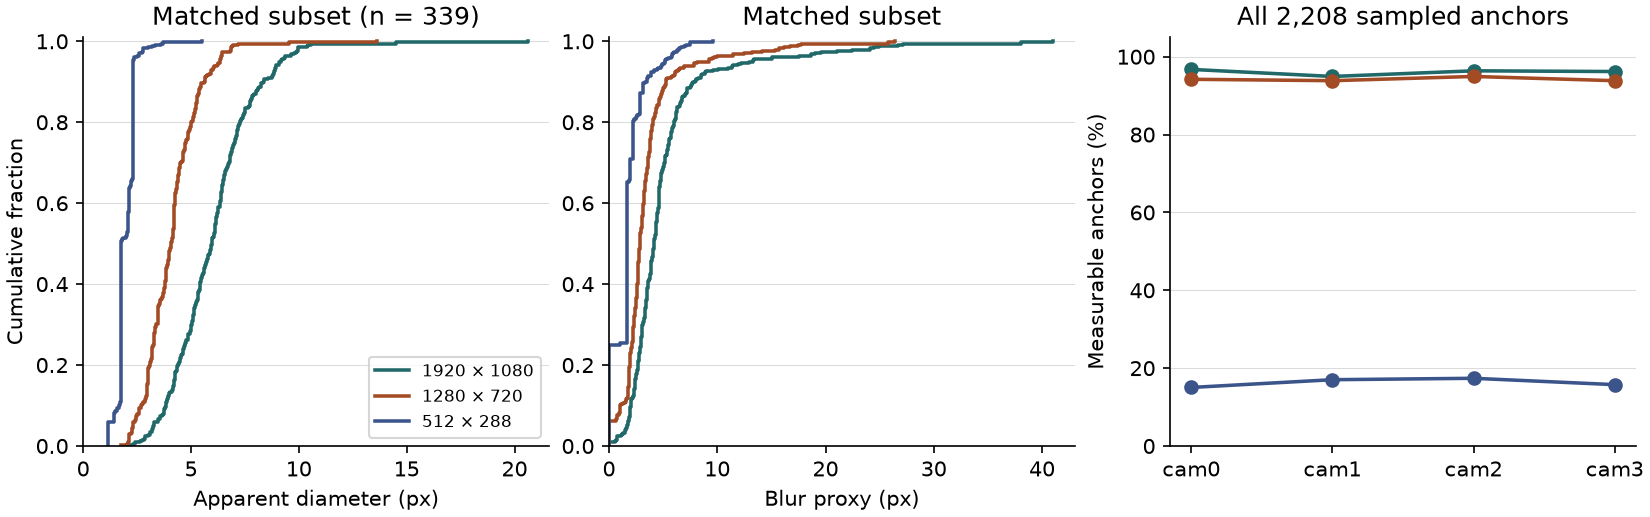
\includegraphics[width=\linewidth]{figures/ball/footprint-distributions.png}
\caption{外部座標付近で測った球像の径と見かけの伸び。左・中央は全サイズで測れた同じ
\ev{ball-footprint}{339}件の累積分布（測定画像px）。右は抽出した\ev{ball-footprint}{2,208}件での視点別の計測成立率。}
\label{fig:ball-footprints}
\end{figure}

\begin{table}[tbp]
\centering
\caption{Meiji 4camの視点別診断。径・伸びは元画像で計測成立した成分の中央値。
範囲外座標は各視点の\ev{ball-visibility}{46,228}座標、可視確認は層化抽出した各視点の\ev{ball-visibility}{16}件を分母とする。}
\label{tab:ball-cameras}
\small
% Generated by scripts/make_tables.py.
\begin{tabular}{@{}lrrrrr@{}}
\toprule
視点 & 計測成立 & 径 [px] & 伸び [px] & 範囲外座標 & 可視確認 \\
\midrule
cam0 & \ev{ball-footprint}{534/552} & \ev{ball-footprint}{3.94} & \ev{ball-footprint}{2.55} & \ev{ball-visibility}{688} & \ev{ball-visibility}{6/16} \\
cam1 & \ev{ball-footprint}{524/552} & \ev{ball-footprint}{3.71} & \ev{ball-footprint}{2.67} & \ev{ball-visibility}{630} & \ev{ball-visibility}{9/16} \\
cam2 & \ev{ball-footprint}{532/552} & \ev{ball-footprint}{4.20} & \ev{ball-footprint}{2.90} & \ev{ball-visibility}{756} & \ev{ball-visibility}{6/16} \\
cam3 & \ev{ball-footprint}{531/552} & \ev{ball-footprint}{4.19} & \ev{ball-footprint}{2.42} & \ev{ball-visibility}{2,062} & \ev{ball-visibility}{6/16} \\
\bottomrule
\end{tabular}

\end{table}

初版の視点・フレーム別外部座標で、画像境界の外に中心があるのは
\ev{ball-visibility}{4,136/184,912}件（\ev{ball-visibility}{2.24\%}）だった。
うち\ev{ball-visibility}{4,125}件には推定座標の区分が付いていた。
画像内の観測、その他の画像内、範囲外座標から層化した目視監査では、
\ev{ball-visibility}{64}件のうち可視\ev{ball-visibility}{27}件、遮蔽\ev{ball-visibility}{2}件、
画面内で識別不能\ev{ball-visibility}{11}件、退出を視認した画面外\ev{ball-visibility}{1}件だった。
範囲外座標の\ev{ball-visibility}{16}件中\ev{ball-visibility}{15}件は退出を視認できなかった。
図\ref{fig:ball-visibility}の目視件数は層化した標本に対する値で、座標範囲外の比率とも評価対象が異なる。

\begin{figure}[tbp]
\centering
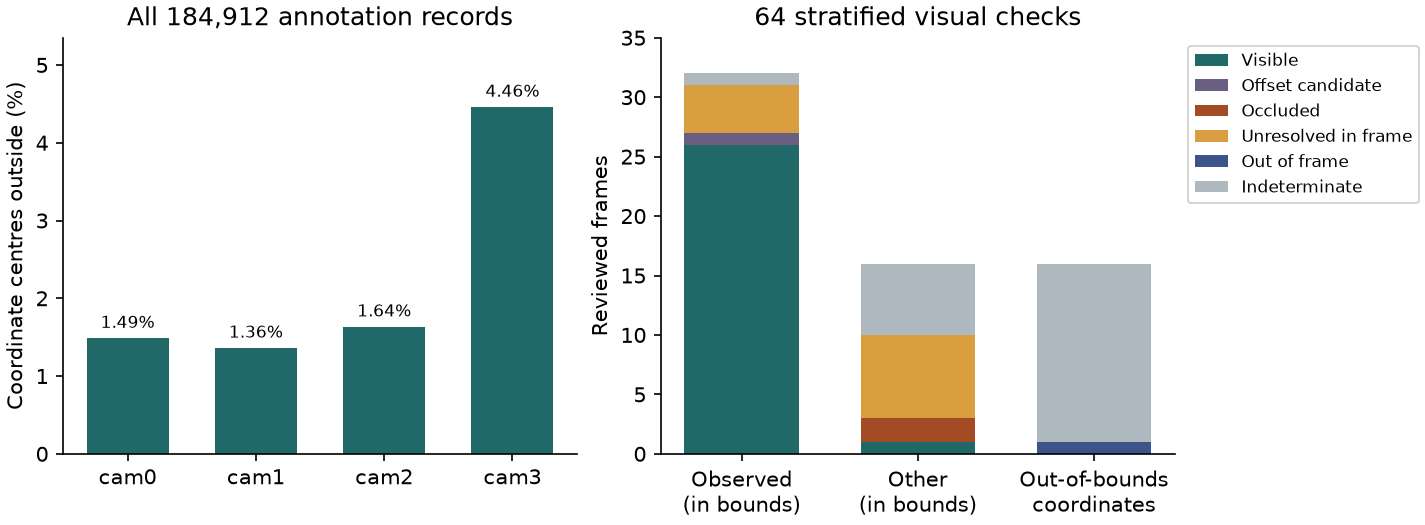
\includegraphics[width=\linewidth]{figures/ball/visibility.png}
\caption{外部座標中心の範囲外率と層化目視監査。座標の全数集計と、映像中で見え方を確認した監査を併記した。}
\label{fig:ball-visibility}
\end{figure}

\subsection{既存の容量・系列長と人工カメラ変動}

球像が縮小で識別しにくくなると、増やしたパラメータがどの程度位置精度に寄与するかは、同じ採点集合で調べる必要がある。
表\ref{tab:ball-history}の容量比較では、共通の長系列validationで最小の約\ev{ball-capacity}{8.0}百万パラメータの条件でも
平均\ev{ball-capacity}{35.38} px、P95 \ev{ball-capacity}{169.69} pxの誤差が残った。
容量を増やした条件で平均は下がったが、誤差分布の裾は大きい。
別の逐次学習のDPT系列では、\ev{ball-length}{32→64}フレームで位置誤差は下がり、更新数は増加した。
また、合成のカメラ変動を加えたConvNeXt＋queryの診断では平均位置誤差が
\ev{ball-camera-stress}{15.4→32.2}元画像pxへ増えた。これは元画像と座標に同じ画像変換を適用し、
変換後の画面外を採点から外した実験であり、撮影機材だけを入れ替えた測定とは条件が異なる。

\begin{table}[tbp]
\centering
\caption{既存の長系列validationでの代表比較。位置の単位は元画像px、採点対象は\ev{ball-length}{85,473}観測フレーム。
逐次学習の行は累積更新数、容量比較の行はquery学習の更新数を示す。}
\label{tab:ball-history}
\small
% Generated by scripts/make_tables.py.
\begin{tabular}{@{}lrrrrr@{}}
\toprule
条件 & 窓長 & 百万parameter & 更新 & 平均 [px] & P95 [px] \\
\midrule
common-dpt-T32 & \ev{ball-length}{32} & \ev{ball-length}{—} & \ev{ball-length}{10,000} & \ev{ball-length}{42.58} & \ev{ball-length}{248.14} \\
dpt-T64 & \ev{ball-length}{64} & \ev{ball-length}{—} & \ev{ball-length}{16,000} & \ev{ball-length}{36.56} & \ev{ball-length}{183.20} \\
query-T32 & \ev{ball-length}{32} & \ev{ball-length}{—} & \ev{ball-length}{16,000} & \ev{ball-length}{42.99} & \ev{ball-length}{136.21} \\
query-T64 & \ev{ball-length}{64} & \ev{ball-length}{—} & \ev{ball-length}{22,000} & \ev{ball-length}{28.20} & \ev{ball-length}{116.89} \\
d256-L4 & \ev{ball-capacity}{64} & \ev{ball-capacity}{8.0} & \ev{ball-capacity}{12,000} & \ev{ball-capacity}{35.38} & \ev{ball-capacity}{169.69} \\
d384-L4 & \ev{ball-capacity}{64} & \ev{ball-capacity}{13.3} & \ev{ball-capacity}{12,000} & \ev{ball-capacity}{35.11} & \ev{ball-capacity}{167.50} \\
d512-L4 & \ev{ball-capacity}{64} & \ev{ball-capacity}{21.0} & \ev{ball-capacity}{12,000} & \ev{ball-capacity}{33.58} & \ev{ball-capacity}{164.14} \\
d768-L4 & \ev{ball-capacity}{64} & \ev{ball-capacity}{41.9} & \ev{ball-capacity}{12,000} & \ev{ball-capacity}{33.88} & \ev{ball-capacity}{160.81} \\
d1024-L4 & \ev{ball-capacity}{64} & \ev{ball-capacity}{71.8} & \ev{ball-capacity}{12,000} & \ev{ball-capacity}{33.38} & \ev{ball-capacity}{161.51} \\
d512-L6 & \ev{ball-capacity}{64} & \ev{ball-capacity}{29.7} & \ev{ball-capacity}{12,000} & \ev{ball-capacity}{34.26} & \ev{ball-capacity}{162.06} \\
d512-L8 & \ev{ball-capacity}{64} & \ev{ball-capacity}{38.3} & \ev{ball-capacity}{12,000} & \ev{ball-capacity}{32.48} & \ev{ball-capacity}{149.47} \\
\bottomrule
\end{tabular}

\end{table}

\subsection{学習済みモデルへの時間文脈の介入}

固定validationから\ev{ball-intervention}{144}アンカーを選び、球を観測した\ev{ball-intervention}{88}件で位置精度を測った。
同じチェックポイント・アンカー・存在閾値で、通常の時系列、アンカー画像の反復、周辺画像をシャッフルする条件を比較した。
RGBからMDDを作る処理は全条件で同じで、アンカーの位置も固定した。
形状ベースの対照では局所コントラスト、丸さ、白・黄の色、背景差分を使い、別収録群で存在閾値を選んだ。

表\ref{tab:ball-intervention}では、位置が\ev{ball-intervention}{20}元画像px以内の件数が、
X3D T32で通常\ev{ball-intervention}{76/88（86.36\%）}から反復\ev{ball-intervention}{2/88（2.27\%）}へ、
i935 T8で通常\ev{ball-intervention}{73/88（82.95\%）}から反復\ev{ball-intervention}{0/88}へ落ちた。
周辺の順序を変えた場合も、全体では両モデルで命中数が減った。形状対照は\ev{ball-intervention}{7/88（7.95\%）}で、
欠測や背景の紛らわしい像も含めたこの集合では、形状と短い背景差分の組合せから球を分けるのが難しかった。

\begin{table}[tbp]
\centering
\caption{固定アンカーに対する推論時の介入。位置は存在閾値を適用する前の予測で採点し、
存在の偽陽性は確認不在\ev{ball-intervention}{56}件、偽陰性は観測\ev{ball-intervention}{88}件を分母とする。
X3Dと形状対照は\ev{ball-intervention}{1280×720}、i935は\ev{ball-intervention}{512×288}。}
\label{tab:ball-intervention}
\small
% Generated by scripts/make_tables.py.
\begin{tabular}{@{}llrrrrr@{}}
\toprule
モデル & 入力 & 平均 [px] & P95 [px] & 命中 & FPR [\%] & FNR [\%] \\
\midrule
X3D T32 & 通常 & \ev{ball-intervention}{24.22} & \ev{ball-intervention}{66.31} & \ev{ball-intervention}{76/88} & \ev{ball-intervention}{21.43} & \ev{ball-intervention}{14.77} \\
X3D T32 & 同一画像を反復 & \ev{ball-intervention}{253.86} & \ev{ball-intervention}{699.98} & \ev{ball-intervention}{2/88} & \ev{ball-intervention}{0.00} & \ev{ball-intervention}{100.00} \\
X3D T32 & 周辺の順序入替え & \ev{ball-intervention}{88.48} & \ev{ball-intervention}{510.17} & \ev{ball-intervention}{55/88} & \ev{ball-intervention}{17.86} & \ev{ball-intervention}{34.09} \\
i935 T8 & 通常 & \ev{ball-intervention}{34.94} & \ev{ball-intervention}{230.85} & \ev{ball-intervention}{73/88} & \ev{ball-intervention}{14.29} & \ev{ball-intervention}{17.05} \\
i935 T8 & 同一画像を反復 & \ev{ball-intervention}{233.16} & \ev{ball-intervention}{494.07} & \ev{ball-intervention}{0/88} & \ev{ball-intervention}{0.00} & \ev{ball-intervention}{100.00} \\
i935 T8 & 周辺の順序入替え & \ev{ball-intervention}{58.01} & \ev{ball-intervention}{302.58} & \ev{ball-intervention}{67/88} & \ev{ball-intervention}{14.29} & \ev{ball-intervention}{36.36} \\
形状対照 & 色・丸さ・背景差分 & \ev{ball-intervention}{458.73} & \ev{ball-intervention}{987.17} & \ev{ball-intervention}{7/88} & \ev{ball-intervention}{62.50} & \ev{ball-intervention}{40.91} \\
\bottomrule
\end{tabular}

\end{table}

\subsection{同一予算での単フレーム学習と時系列学習}

推論時の反復に加え、各入力で最初から学習し直した。同じX3D／CSN＋DPTを
\ev{ball-train-plan}{512×288}、seed \ev{ball-train-plan}{42}、
\ev{ball-train-plan}{30,478}学習パックで比較し、初期重みの共通部分と抽出順を揃えた。
各条件は\ev{ball-train-plan}{4,700}更新、更新当たり\ev{ball-train-plan}{128}枚、計\ev{ball-train-plan}{601,600}入力フレームだった。
単フレームにはRGBを、時系列にはRGBと各窓から計算したMDDを入力した。

全validationの\ev{ball-train-val}{117,358}件（observed \ev{ball-train-val}{85,473}件）では、
\ev{ball-train-val}{20} px以内率が単フレームRGBの\ev{ball-train-val}{1.66\%}から、
\ev{ball-train-plan}{T=8}で\ev{ball-train-val}{40.90\%}、\ev{ball-train-plan}{T=32}で\ev{ball-train-val}{44.23\%}に上がった。
Chat、Meiji 3cam、TrackNet game9のすべてで上がり、同じ\ev{ball-train-anchor}{144}アンカーでも
\ev{ball-train-anchor}{2/88→40/88→45/88}と増えた（表\ref{tab:ball-training}、図\ref{fig:ball-training}）。
存在F1は各条件のvalidationでFPRとFNRの平均が最小となる閾値で集計した。位置採点にはこの閾値を適用しない。

単フレームからの差にはMDDの有無が含まれる。
両方でRGB＋MDDを使う\ev{ball-train-plan}{T=8とT=32}の比較では、
窓の延長に伴う改善は全validationで\ev{ball-train-val}{3.33}ポイント、アンカーで\ev{ball-train-anchor}{5.68}ポイントだった。
単一seed・固定解像度での結果で、独立testは今後の評価に含める。
この学習比較と前節のチェックポイント比較では、学習履歴と入力解像度が異なる。

\begin{table}[tbp]
\centering
\caption{入力条件ごとに学習した検出器の成績。位置誤差はobservedの元画像px。
収録元別の\ev{ball-train-val}{20} px以内率の分母は、Chat \ev{ball-train-sources}{61,369}件、
Meiji 3cam \ev{ball-train-sources}{23,007}件、TrackNet game9 \ev{ball-train-sources}{1,097}件。}
\label{tab:ball-training}
\small
% Generated by scripts/make_tables.py.
\begin{tabular}{@{}lrrr@{}}
\toprule
指標 & \ev{ball-train-plan}{T=1} RGB & \ev{ball-train-plan}{T=8} RGB＋MDD & \ev{ball-train-plan}{T=32} RGB＋MDD \\
\midrule
平均位置誤差 [px] & \ev{ball-train-val}{226.75} & \ev{ball-train-val}{134.06} & \ev{ball-train-val}{125.74} \\
中央値位置誤差 [px] & \ev{ball-train-val}{177.02} & \ev{ball-train-val}{42.48} & \ev{ball-train-val}{31.68} \\
全validationの命中率 [\%] & \ev{ball-train-val}{1.66} & \ev{ball-train-val}{40.90} & \ev{ball-train-val}{44.23} \\
存在F1 [\%] & \ev{ball-train-val}{74.07} & \ev{ball-train-val}{82.02} & \ev{ball-train-val}{82.63} \\
Chatの命中率 [\%] & \ev{ball-train-sources}{1.29} & \ev{ball-train-sources}{45.54} & \ev{ball-train-sources}{49.20} \\
Meiji 3camの命中率 [\%] & \ev{ball-train-sources}{2.66} & \ev{ball-train-sources}{27.36} & \ev{ball-train-sources}{29.77} \\
TrackNet game9の命中率 [\%] & \ev{ball-train-sources}{1.37} & \ev{ball-train-sources}{65.18} & \ev{ball-train-sources}{69.10} \\
固定アンカーの命中数（率 [\%]） & \ev{ball-train-anchor}{2/88（2.27）} & \ev{ball-train-anchor}{40/88（45.45）} & \ev{ball-train-anchor}{45/88（51.14）} \\
\bottomrule
\end{tabular}

\end{table}

\begin{figure}[tbp]
\centering
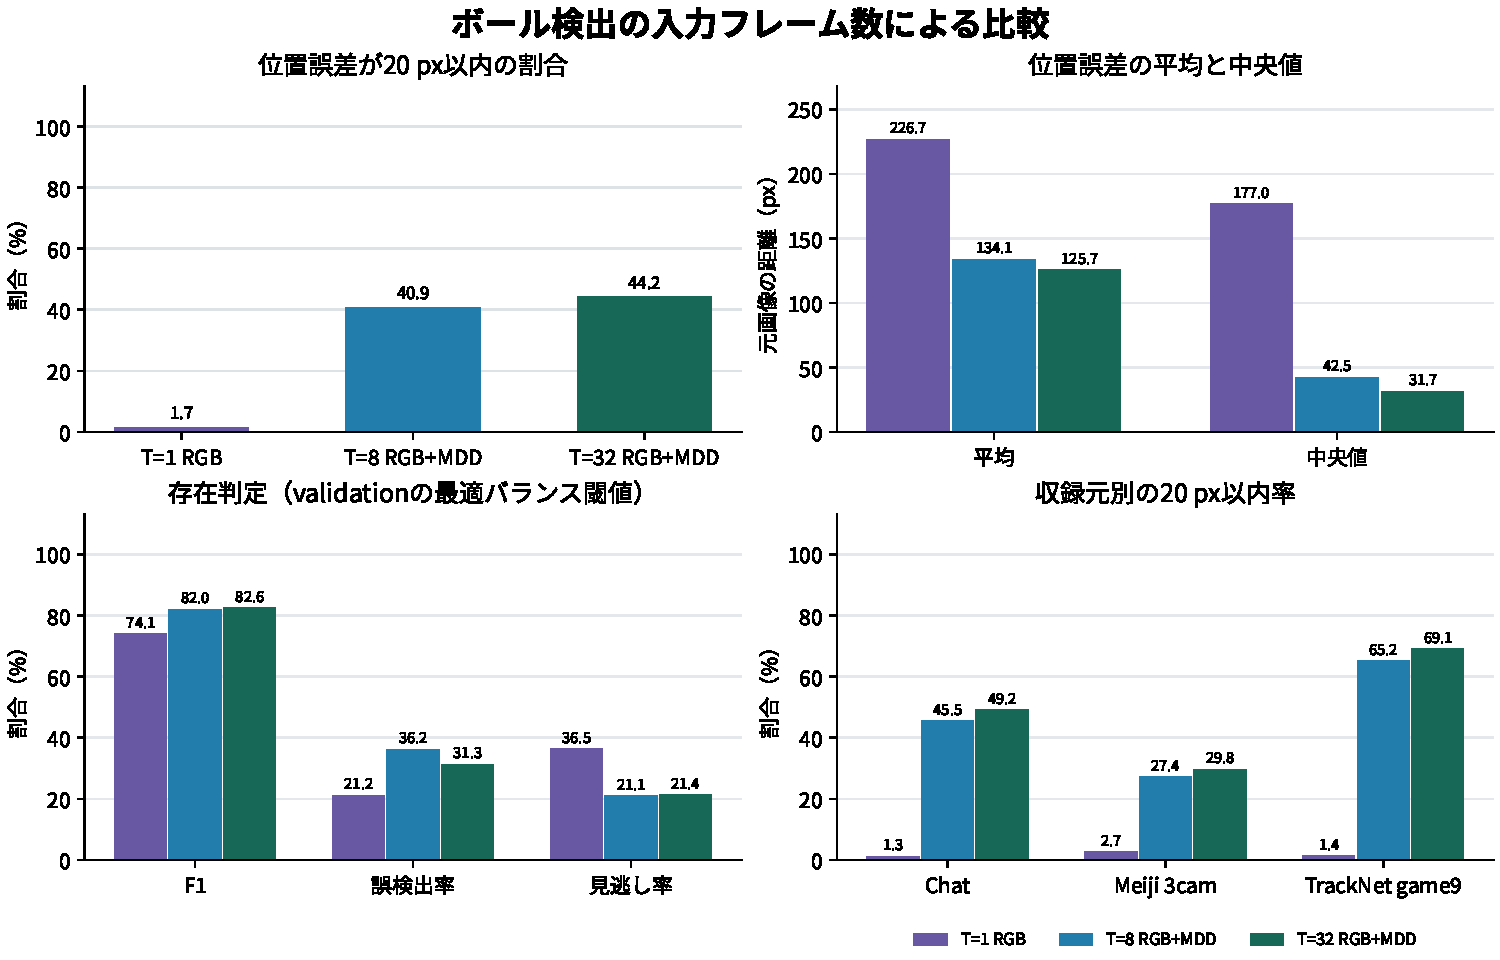
\includegraphics[width=\linewidth]{figures/ball/temporal_training_ablation.pdf}
\caption{同一学習予算での全validationの比較。位置は元画像px、存在F1は全validationで選んだ閾値を用いた。}
\label{fig:ball-training}
\end{figure}
\FloatBarrier
